% CipherScope manuscript. CANONICAL SOURCE (manuscript.md is superseded).
% Structure follows the dominant flow of 10 reference FHE-systems papers:
%   Intro -> Background and Motivation -> Threat Model and Scope ->
%   Framework -> Experimental Setup -> Results and Discussion ->
%   Limitations -> Related Work -> Conclusion and Future Work.
% Build: cd paper && tectonic manuscript.tex
% Figures: python3 figures/make_figures.py (from evaluation/tables/*.csv);
%          tectonic figures/teaser.tex -o figures   (TikZ overview diagram)
% For double-blind submission, add [review,anonymous] back to the class options.
\documentclass[sigconf,nonacm]{acmart}

\usepackage{booktabs}
\usepackage{xcolor}
\usepackage{microtype}
% Long identifiers like GetCryptoContext() otherwise overflow the narrow
% column. Extra emergency stretch lets TeX loosen a line rather than let it
% run into the gutter; \code is \texttt with break opportunities at the
% word boundaries of a CamelCase identifier.
\setlength{\emergencystretch}{3em}
\newcommand{\code}[1]{\texttt{#1}}

% Marker for open items; currently unused (all resolved or stated in prose).
\newcommand{\verify}[1]{\textcolor{red!70!black}{\footnotesize [VERIFY: #1]}}

\settopmatter{printacmref=false}
\renewcommand\footnotetextcopyrightpermission[1]{}
\pagestyle{plain}

\begin{document}

\title{CipherScope: Runtime Semantic Observability and Diagnosis for OpenFHE Programs}

\author{Kimon Antonios Provatas}
\affiliation{\institution{The University of Texas at Austin}\city{Austin}\state{Texas}\country{USA}}

\author{Ilias Georgakopoulos-Soares}
\affiliation{\institution{The University of Texas at Austin}\city{Austin}\state{Texas}\country{USA}}

\author{Karim Benhamou}
\affiliation{\institution{The University of Texas at Austin}\city{Austin}\state{Texas}\country{USA}}

\begin{abstract}
Developers of fully homomorphic encryption (FHE) applications work largely
blind: a conventional profiler reports where time is spent, but the decisions
that determine an encrypted program's cost and correctness---whether rotations
share a ciphertext, whether generated keys are ever used, how much of the
multiplicative-depth budget an execution actually consumes---depend on
semantic facts that timing alone cannot express. We present CipherScope, a
runtime observability and diagnosis system for OpenFHE programs. CipherScope
traces a program at its application boundary, through a Python proxy or a GCC
compiler plugin for unmodified C++ programs, and reconstructs the execution
into a validated graph of immutable ciphertext versions, per-scheme state
transitions, and provenance. Conservative rules over this graph report
candidate optimizations and misconfigurations, each carrying the evidence
that triggered it, and each abstaining with a stated reason when its
preconditions are unobserved. The observation boundary itself is measured:
every run receives a coverage class, and only completely observed runs enter
quality claims. We evaluate fidelity, coverage, finding quality, impact, and
cost across CKKS, BFV, and BGV: tracing preserves program output; a
known-answer benchmark yields perfect recall with no false positives on hard
negatives; and on an independently authored workload corpus, six of eight
adjudicated findings were actionable---acting on them produced speedups of up
to 4$\times$ and surfaced measured security--performance trades---while
tracing adds under 2\% overhead on realistic workloads. The principal
limitation is the observation boundary itself, which we quantify rather than
assume away.
\end{abstract}

\maketitle

\section{Introduction}
\label{sec:intro}

Consider an OpenFHE program that encrypts a packed vector, rotates the
ciphertext by four different indices, and combines the results. A line-level
profiler reports that the four \texttt{EvalRotate} calls dominate the run
time. The developer who wants to act on that observation needs answers to
questions the profile does not contain. Did all four rotations read the
\emph{same} recorded ciphertext version, so that a single hoisted
precomputation could serve them all? Is the context's key-switching technique
one under which that shared precomputation is known to reproduce the regular
rotation exactly? Was one of the rotation keys generated at setup never used
by the executed run, wasting key-generation time and memory? None of these
are timing facts. They are facts about ciphertext identity, library
configuration, and executed provenance, and they are exactly what a
conventional profile discards.

CipherScope is a runtime observability and diagnosis system for OpenFHE
programs~\cite{openfhe2022} that records these facts while the program runs.
It observes the application's own calls into OpenFHE---not the library's
internals---and builds an explicit model of the execution: every covered call
attributed to its source line, every ciphertext result assigned an immutable
version identifier, every in-place mutation producing a new version, and
every version carrying the state its scheme exposes (level, scale, noise
degree, slot count, key tag, key-switching technique). Rules over the
resulting graph report findings such as ``these four rotations read
ciphertext version \texttt{ct\_0001:v0} under BV key switching and no
compatible precomputation precedes them,'' each tied to the evidence events
and source lines that justify it.

Three design decisions distinguish CipherScope from both profilers and FHE
compilers. First, the unit of observation is the application-level semantic
call, not a native kernel or a compiler intermediate representation:
CipherScope answers questions about the program the developer wrote and ran,
including branches a compiler cannot see taken and configurations fixed only
at run time. Second, the rules are deliberately conservative: each fires only
on recorded evidence and explicit developer assertions, abstains with a
stated reason when its preconditions are unobserved, and recommends a
measured experiment rather than promising a speedup. Third, the observation
boundary is itself measured: every run receives a coverage class
(\texttt{COMPLETE}, \texttt{PARTIAL-PERMISSIVE}, or \texttt{UNSUPPORTED}),
and only \texttt{COMPLETE} runs enter any quality claim in this paper.

The same canonical trace is produced by two frontends. The Python frontend
wraps a live crypto context in a proxy; a runner intercepts the program's
\texttt{GenCryptoContext} call so that existing scripts run unmodified. The
C++ frontend is a GCC plugin that instruments the OpenFHE call boundary of an
unmodified program in a shadow build, leaving the source tree and the
original binary untouched. Validation, the ciphertext graph, all twelve
rules, and every exporter are shared; a gate check asserts that the C++ and
Python traces of twin programs are semantically equivalent.

This paper makes four contributions.

\begin{enumerate}
\item \textbf{A source-attributed runtime model of FHE execution}
  (\S\ref{sec:framework}): immutable ciphertext versions, per-scheme state
  transitions, rotation-key use, and lineage, reconstructed from covered
  calls into a validated graph, with the observation boundary explicit and
  measured. The model is scheme-parametric: CKKS, BFV, and BGV are identified
  from a live context with no declared parameters, and multiplicative depth
  is read from whichever coordinate the scheme actually moves---the level
  ladder for CKKS and BGV, and the recorded multiplication count for BFV,
  whose level never changes and whose noise-scale degree we measured to be
  non-cumulative (\S\ref{sec:scheme}).
\item \textbf{Conservative diagnosis rules over that model}
  (\S\ref{sec:rules}): twelve rules covering repeated compatible rotations,
  rotation keys unused in the observed run, observed depth headroom,
  bootstrap restoration use, annotated packing utilization, public-value
  provenance, repeated public encodings, serial associative reductions,
  precision checkpoints and declared tolerances, testing-only security
  configuration, and the depth critical path.
\item \textbf{An evidence methodology for FHE tooling} (\S\ref{sec:setup}):
  coverage classes that keep incompletely observed runs out of quality
  claims; a seeded known-answer benchmark with hard negatives for recall;
  adjudication of every real finding under a fixed rubric for precision;
  before/after patches for every actionable finding; and a data contract
  under which every table in this paper regenerates byte-identically from
  checksummed raw records.
\item \textbf{Measured results on real workloads} (\S\ref{sec:results}): on
  an independently authored corpus, six of eight adjudicated findings were
  actionable; all six patches were applied and measured---three performance
  findings at 1.09$\times$--4.03$\times$, and three security-enforcement
  fixes whose measured outcomes range from free to a 4$\times$ slowdown with
  changed results, reported as the trade they are---and the two false
  positives are analyzed rather than discarded: one exposed a missing level
  reservation that is now part of the depth-headroom rule.
\end{enumerate}

We do not claim that CipherScope is the first FHE profiler, that it replaces
compilers or library benchmarks, or that its suggestions are guaranteed
improvements. \S\ref{sec:related} positions it against systems that answer
adjacent questions; \S\ref{sec:limits} states what it cannot see.

\section{Background and Motivation}
\label{sec:background}

\subsection{Fully homomorphic encryption and the three schemes}

FHE evaluates programs over encrypted data. The schemes relevant here are
CKKS~\cite{ckks2017}, which computes on encrypted fixed-point-like
approximations of real vectors, and BFV~\cite{brakerski2012,fv2012} and
BGV~\cite{bgv2012}, which compute exactly on packed integer vectors modulo a
plaintext modulus $t$. Three properties drive the diagnostics in this paper.

\paragraph{Multiplicative depth is a budget.} A crypto context is configured
with a multiplicative depth; each ciphertext--ciphertext multiplication
consumes from it. In OpenFHE's CKKS and BGV, consumption is visible as a
per-ciphertext \emph{level} that increases monotonically within a bootstrap
epoch. BFV exposes no such ladder (\S\ref{sec:scheme}). Exceeding the budget
does not necessarily raise an error: a BGV result can silently decrypt to a
wrong value, which makes depth accounting a correctness concern rather than
only a performance one.

\paragraph{Rotations need keys, and keys are per index.} Rotating packed
slots by index $i$ requires a rotation key generated for $i$ at setup.
Generating keys for indices the run never uses costs time and memory. Several
rotations of the \emph{same} ciphertext version can share one expensive
precomputation (\texttt{EvalFastRotationPrecompute})---but only of the same
version, and the equivalence of the shared form depends on the key-switching
technique in use.

\paragraph{CKKS is approximate; BFV and BGV are exact.} A CKKS value carries
noise that grows with computation, so precision loss is a measurable,
meaningful quantity. An exact scheme that produces a wrong value has not
``lost precision''; it has failed, typically by exceeding the noise budget or
overflowing $t$. Diagnostics designed for approximation error have nothing to
measure on exact schemes, and the tool must say so rather than report a
vacuously clean result.

\subsection{OpenFHE and the application boundary}

OpenFHE~\cite{openfhe2022} is an open-source C++ FHE library with a Python
wrapper. An application obtains a crypto context from declared parameters,
generates keys, and issues semantic calls (\texttt{Encrypt},
\texttt{EvalAdd}, \texttt{EvalMult}, \texttt{EvalRotate},
\texttt{EvalBootstrap}, \texttt{Decrypt}, and their variants) against that
context. This call surface is the \emph{application boundary}: everything
CipherScope observes crosses it, and everything below it---the library's
number-theoretic transforms, key-switching internals, memory
management---remains opaque by design. Prior work characterizes what happens
below this boundary (\S\ref{sec:related}); CipherScope characterizes the
program above it.

\subsection{A motivating example}
\label{sec:example}

The OpenFHE project ships \texttt{simple-integers.py}, a 103-line BFV example
that encrypts three integer vectors, adds and multiplies them, and rotates
the first ciphertext by indices 1, 2, $-1$, and $-2$. We use it as the
running example because we did not write it, and because tracing it
end-to-end exercises the exact chain of facts the Introduction claims a
profile lacks. Figure~\ref{fig:overview} contrasts what a timing profile
keeps with what CipherScope records for this run.

\begin{figure*}
  \centering
  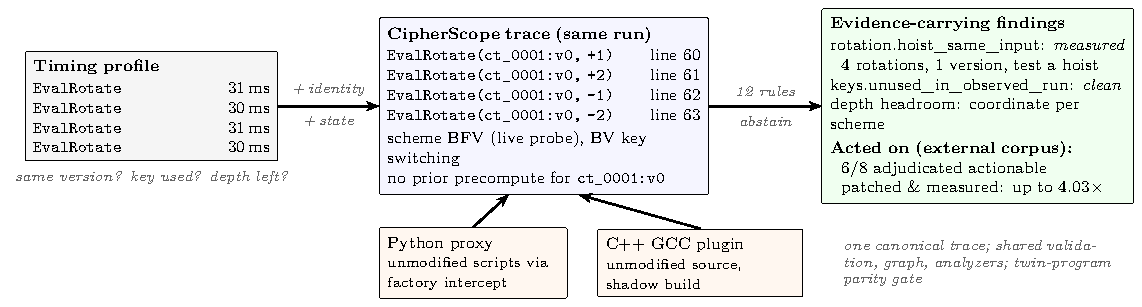
\includegraphics[width=0.92\textwidth]{figures/teaser.pdf}
  \caption{What a timing profile keeps versus what CipherScope records for
  the same four-rotation BFV run (the upstream \texttt{simple-integers.py}
  example of \S\ref{sec:example}), and where the added facts go: a validated
  version/state graph, twelve conservative rules, and---on an independently
  authored corpus---adjudicated findings whose patches were measured. Both
  frontends emit one canonical trace.}
  \label{fig:overview}
\end{figure*}

A timing profile of this program attributes some milliseconds to each
\texttt{EvalRotate} line. CipherScope's trace of the same run records, in
addition: that all four rotations read ciphertext version
\texttt{ct\_0001:v0}; that the requested indices were $\{-2,-1,1,2\}$; that
the context's key-switching technique is BV (the BFV default, unlike the
HYBRID default of CKKS and BGV); and that no
\texttt{EvalFastRotationPrecompute} for that version precedes the group. The
rotation-hoisting rule therefore fires with measured confidence, naming the
four evidence events and the shared source version, and recommends testing a
hoisted precomputation---a recommendation the rule is only entitled to make
under BV because a gate check (\S\ref{sec:rq1}) first established that a
shared precomputation reproduces regular rotations exactly under that
technique. On the same trace the depth-critical-path rule reports the
executed multiplication chain, and the unused-key rule stays silent because
every generated key was used. When we ran this program and its BGV twin
under the tracer, both were completely observed (\texttt{COMPLETE}, 17
semantic calls) with bit-identical decrypted output (\S\ref{sec:rq2}).

This is the pattern for everything that follows: a fact a profile cannot
express, a recorded representation of that fact, a rule that uses it under
stated preconditions, and an abstention path when the preconditions fail.

\section{Threat Model and Scope}
\label{sec:threat}

CipherScope is a development-time tool, and its security story is
deliberately modest. We state it before the design so the reader knows what
the system does and does not promise.

\paragraph{Setting.} A developer traces their own program, in their own
environment, over data they are entitled to see. CipherScope is not deployed
against an adversary; the ``threats'' it addresses are honest mistakes:
inefficient structure, wasted keys, over-provisioned depth, and testing-only
configurations left enabled in programs headed for deployment.

\paragraph{Traces are sensitive artifacts.} A trace records argument and
result representations, exception messages, absolute source paths, and, when
the developer opts into shadow mode by supplying a secret key, the decrypted
values compared at each precision checkpoint. A trace records no key material
and no ciphertext coefficients, but we claim no leakage guarantee, and traces
should be treated as confidential development artifacts, not published
as-is.

\paragraph{No cryptographic security claims.} The configuration rule reports
a declared enforcement setting---a run that declares
\texttt{HEStd\_NotSet} is flagged as a testing-only configuration. This is a
configuration observation. CipherScope never estimates bit security, never
validates parameter choices, and a clean report is not evidence that a
parameter set is secure. Side channels, fault attacks, and the library's own
implementation security~\cite{safetycentric2025} are out of scope.

\paragraph{Observation requires cooperation.} The Python frontend observes
calls that pass through its proxy; the C++ frontend observes calls its
plugin instrumented. A program that routes around either boundary is not
observed, and \S\ref{sec:coverage} describes how that is detected and
classified rather than silently tolerated.

\section{The CipherScope Framework}
\label{sec:framework}

\subsection{Design principles}
\label{sec:principles}

Four ideas determine what CipherScope can say, and each is a deliberate
restriction rather than a feature.

\paragraph{Observe where the decisions are made.} An FHE program's cost is
set by choices the developer controls: which ciphertext an operation reads,
how deep the multiplication chain runs, which keys are generated, what the
context declares. Those choices are expressed at the application boundary
(\S\ref{sec:background}), so that is where CipherScope listens. Watching
further down---inside key switching, inside the number-theoretic
transform---would measure the library's engineering, which the developer
cannot change and other tools already characterize. Watching further up,
before execution, would miss the branch actually taken and the parameters
actually chosen at run time.

\paragraph{Make ciphertext identity explicit.} ``Do these two rotations read
the same ciphertext?'' is the question a profile cannot answer, and it only
becomes answerable once identity is defined. CipherScope treats every
ciphertext value as immutable and names each one: an operation that mutates
its operand in place does not modify a value, it creates the next
\emph{version} of it. Versioning turns a vague question about object
identity into a precise one about recorded lineage, and it is what lets a
rule distinguish four rotations of one version---hoistable---from four
rotations of a value that changed between them.

\paragraph{Treat the trace as a contract.} Acquisition and analysis meet at
one schema-versioned document and nowhere else. This is why a Python proxy
and a GCC compiler plugin, which share no implementation, can feed the same
graph, the same rules, and the same exporters: each frontend's only
obligation is to emit a valid canonical trace. The contract also makes the
evidence auditable---a finding can be traced back to the events that caused
it, and every table in this paper regenerates from archived traces without
rerunning any FHE computation.

\paragraph{Prefer abstention to inference.} A rule fires on recorded
evidence or an explicit developer assertion, never on a guess about
encrypted contents. When a precondition is unobserved, the rule abstains and
says which one, rather than defaulting to a clean result that reads like
evidence of absence. For the same reason a finding recommends an experiment
and reports the stake---the combined time of the rotations in question---in
place of a predicted speedup the tool is in no position to promise. The
cost of this stance is visible in our own numbers: rules abstain on many
real runs (\S\ref{sec:rq6}), and we count that rather than hide it.

\subsection{Canonical trace and ciphertext versioning}
\label{sec:trace}

A run produces a validated bundle: a schema-versioned trace (events,
ciphertext versions, context description, coverage record), a derived
ciphertext graph, rule findings, and exporters (CSV, Perfetto, a static HTML
report). Each event records the operation's canonical name, its source
attribution (file, line, function, call-site identifier), wall and
process-CPU duration for the whole call, input and output ciphertext
versions with their state snapshots, semantic arguments (for example, the
requested rotation index), and status---a failing call becomes an error
event rather than a gap.

Ciphertext identity is version-based. A ciphertext result is assigned an
identifier such as \texttt{ct\_0002:v0}; an in-place operation
(\texttt{EvalAddInPlace}, \texttt{RescaleInPlace}) produces the next version
of its operand, and later reads observe the new version. Aliasing---handle
copies, moves, container storage---preserves identity; destroyed objects
never leak their identifier to a reused address. These properties are
asserted by gate checks against the real library, not assumed.

Recording is bounded: events and finalized ciphertext states spool to disk
during the run, and hard limits on event count and trace size stop recording
(never the workload) and mark the trace truncated. Finalization is not
streamed: building and analyzing the trace materializes it, at about
2.2\,KB of trace and 30\,KB of peak memory per event (\S\ref{sec:rq5}).

\subsection{Two frontends, one canonical trace}
\label{sec:frontends}

The \textbf{Python frontend} wraps a native crypto context in a proxy. Only
calls through the proxy are observed. In strict mode, a call the
compatibility registry cannot classify is rejected and named; in permissive
mode it is forwarded and the trace is marked incomplete. The runner executes
an unmodified script by intercepting its \texttt{GenCryptoContext} call and
attaching the returned context, so corpus workloads run without edits;
programs that obtain contexts by other means must attach them explicitly.

The \textbf{C++ frontend} is a GCC plugin. \texttt{cipherscope profile
<binary>} discovers the target's CMake build, creates an instrumented
\emph{shadow} build without touching the source tree or the original binary,
and the plugin instruments each application-boundary OpenFHE call site
during compilation. Instrumentation precedes optimization: a gate check
asserts that the same events and source lines are recorded at \texttt{-O0},
\texttt{-O2}, and \texttt{-O3}. Operator overloads ($*$, $+$, $+{=}$, unary
$-$) normalize to the same canonical events as named calls; concurrent calls
from OpenMP threads are recorded once each. The spooled native trace is
normalized into the same canonical schema the Python frontend emits, and the
entire downstream pipeline---validation, graph, rules, exporters---is
shared. A parity gate check asserts that C++ traces of eight twin programs
are semantically equivalent to the Python frontend's traces of the same
computations.

\subsection{Coverage classification}
\label{sec:coverage}

Because the tool cannot see calls that bypass the application boundary,
every run is classified. \texttt{COMPLETE} requires strict mode, a finished
run, at least one traced semantic call, nothing forwarded untraced, and no
bypass pattern in the target's source (a preflight scan of the program's
syntax tree looks for raw-context use, module-level \texttt{Eval*} free
functions, and \texttt{GetCryptoContext()} escapes).
\texttt{PARTIAL-PERMISSIVE} and \texttt{UNSUPPORTED} runs are excluded from
every quality claim. The classification is operational, not a proof: a clean
scan does not demonstrate the absence of every possible bypass, and we state
it as such.

Rejections are informative. When we traced the five upstream OpenFHE
integer-scheme examples (\S\ref{sec:rq2}), three were rejected in strict
mode, naming \texttt{MultipartyKeyGen} and \texttt{ReKeyGen}---the
threshold-FHE and proxy-re-encryption families, which the operation manifest
does not cover. The failure mode is the designed one: the unsupported
operation is named in the coverage record rather than silently forwarded.

\subsection{A scheme-parametric state model}
\label{sec:scheme}

The trace records the scheme, and the rules read state through it. Three
measured facts on the pinned build shape the model; none is documented
behavior we could have assumed.

\paragraph{Scheme identification without declared parameters.} The Python
wrapper exposes no scheme getter. CipherScope identifies CKKS by probing
\texttt{GetModulusCKKS()}, which answers for a CKKS context and raises for
the integer schemes; among the rest, only BFV runs with the
\texttt{NORESCALE} scaling technique, which separates it from BGV. Declared
parameters, when present, take precedence, and the trace records which
evidence named the scheme. A gate check holds this for all three schemes
across the supported scaling techniques.

\paragraph{BFV has no level ladder, and its noise-scale degree is not a
substitute.} \texttt{GetLevel()} returns 0 for every BFV ciphertext in a
run. The noise-scale degree looks like a replacement---it is 1 on a fresh
ciphertext and rises by one per multiplication---but it is not cumulative:
measured on the pinned build, \texttt{EvalAdd} of a degree-1 and a degree-2
ciphertext returns degree~1, erasing the record of the multiplication
upstream. Our first implementation used the degree and was caught not by our
seeded cases (pure multiplication chains, which the degree tracks) but by a
C++ twin program whose final addition mixes depths. BFV depth is therefore
counted from the recorded multiplications along the deepest lineage, every
depth finding names its coordinate (\texttt{ciphertext\_levels} or
\texttt{recorded\_multiplications}), and BFV findings carry inferred rather
than measured confidence.

\paragraph{BFV's configured depth is a noise budget, not a multiplication
counter.} On the pinned build, a depth-2 BFV context completed three
successive multiplications correctly, and depth 2 and depth 3 had the same
capacity for the operands we tested; capacity is value-dependent, and
exceeding it decrypts to a wrong plaintext without raising. The BFV
depth-headroom finding therefore carries explicit limitations saying exactly
this, and its numeric headroom is an inference about the observed inputs,
not a measurement of a ladder.

Where the schemes are uniform, the model says so: BGV spends levels exactly
as CKKS does (one per multiplication, same minimum depth across all four
scaling techniques we tested), packing capacity is $N$ slots for the integer
schemes versus $N/2$ for CKKS, and bootstrapping is unavailable for BFV and
BGV on this build (\texttt{EvalBootstrapSetup} raises ``Not supported''),
which the bootstrap rule reports as its reason for abstaining.

\subsection{Diagnosis rules}
\label{sec:rules}

Each rule states its preconditions, the evidence it records, the diagnosis,
and the experiment it suggests; each abstains with a stated reason when a
precondition is unobserved. We describe four in detail and summarize the
rest; \S\ref{sec:rq3} evaluates all twelve.

\paragraph{Repeated compatible rotations.} Fires when at least two
\texttt{EvalRotate} calls with distinct requested indices read the same
ciphertext version, their context, key tag, scaling state, and key-switching
technique match, the technique is one for which shared precomputation has
gate-check equivalence evidence (HYBRID and BV), no compatible
precomputation precedes the group, and no in-place mutation intervenes. The
suggestion is to test a hoisted precomputation; the finding reports the
combined wall time of the group as the stake, not a predicted saving. The
rule abstains, naming the ciphertext, when metadata is missing or the
technique lacks evidence.

\paragraph{Rotation keys unused in the observed run.} Compares the indices
requested at key generation against the indices of executed rotations and
reports the difference. The scope is deliberately ``in the observed run'': a
key unused on this input may be needed on another, and the finding says so.

\paragraph{Observed depth headroom.} Compares the configured multiplicative
depth against the executed depth requirement, read from the scheme's
coordinate (\S\ref{sec:scheme}), and reserves one level when the deepest
ciphertext still carries a deferred rescale---a reservation added after an
adjudicated false positive showed the level field lagging a committed level
(\S\ref{sec:rq3b}). It abstains when the depth model is not fully resolved,
for example when an opaque call (\texttt{EvalChebyshevSeries},
\texttt{EvalLogistic}) hides part of the path. Headroom is an upper bound:
levels a library call consumes internally are not observed, and the
finding's limitations say so.

\paragraph{Testing-only security configuration.} The security level is not
readable from a live context, so this rule assesses only runs that declare
their parameters; it reports a declared \texttt{HEStd\_NotSet} as a
testing-only configuration (\S\ref{sec:threat}). It abstains on undeclared
runs rather than inferring from ring size.

The remaining rules follow the same contract. Bootstrap restoration reports
a bootstrap that restored more levels than its epoch then consumed; it
requires an input deeper than the fixed level OpenFHE returns every
bootstrap output at, and it abstains on BFV and BGV with the measured ``Not
supported'' reason. Packing utilization, public-value provenance, and
repeated public encodings fire only on explicit developer annotations
(declared meaningful slots, declared provenance, declared constant
identity)---CipherScope never infers semantic content from ciphertexts.
Serial reduction review fires only inside regions the developer declares
associative. The two precision rules require shadow mode with a supplied
secret key; checkpoint drops below 3.0 absolute bits are ignored because
CKKS decryption is noise-flooded (measured jitter standard deviation 0.68
bits; an earlier 1.0-bit threshold produced a ${\sim}5\%$ false-positive
rate on noise alone), and both rules abstain on the exact schemes. The depth
critical path is informational: it always reports when lineage exists and is
not counted in precision (\S\ref{sec:rq3b}).

\section{Experimental Setup}
\label{sec:setup}

\paragraph{Research questions.} RQ1: does tracing preserve program behavior
and reconstruct state correctly, on every supported scheme? RQ2: what
fraction of real workloads is completely observed? RQ3: what are recall on
known-answer programs and precision on real findings? RQ4: do validated
findings produce measured improvements? RQ5: what does tracing cost? RQ6:
does the tool expose real misconfigurations?

\paragraph{Pinned build and evidence lanes.} All results use OpenFHE~1.5.1
with Python wrapper 1.5.1.0, pinned by commit. An \emph{evidence lane} is
one exact combination of operating system, toolchain, and build on which the
integration gate ran: the authoritative lane is an Ubuntu 24.04 x86\_64
container (GCC 13.3) built and run on a TACC Lonestar6 node; supporting
lanes are a bare-metal Rocky Linux 8.10 build (GCC 15.2), a macOS arm64
developer build, and an x86\_64 Docker lane run under emulation. Every lane
archives a feasibility artifact with the native-module hashes that tie any
run bundle to the build that produced it.

\paragraph{Corpora.} Four bodies of programs back the claims. (1) A
\emph{seeded benchmark} of 61 known-answer cases (28 CKKS, 17 BFV, 16 BGV):
for each rule, cases that must fire and hard negatives that must not, with
every expected number hand-derivable from the case's source. (2) A
\emph{CKKS corpus} of 16 gallery examples plus the four workloads of an
independently authored regression suite, pinned by commit. (3) An
\emph{integer-scheme corpus}: the five BFV/BGV examples shipped inside the
pinned OpenFHE wrapper itself. (4) A \emph{designed impact suite} pairing
every prescriptive rule with a minimal program, a patch following the rule's
suggestion, and a re-trace.

\paragraph{Adjudication protocol.} Every finding from every completely
observed run of the CKKS corpus was exported and judged under a fixed
rubric. Adjudication was performed by two AI reviewers, not humans: a first
pass, then a blind second pass by a different model with no access to the
first verdicts and the ability to run depth-reduction experiments on a
scratch copy of the corpus. Disagreements were resolved toward the reviewer
who executed the experiment. We state this plainly as a methodological
limit: the rubric, verdicts, and experiment transcripts are in the artifact,
and nothing prevents re-adjudication by humans.

\paragraph{Reproducibility contract.} Every table and figure in this paper
regenerates from checksummed raw records via deterministic generators;
regeneration is byte-identical and asserted by a test. Figures are produced
by a script that reads only the generated tables, so no number is
transcribed by hand.

\section{Results and Discussion}
\label{sec:results}

Table~\ref{tab:summary} collects the headline result for each research
question with its population; the subsections below explain what each
result does and does not establish.

\begin{table}
  \caption{Headline results and their populations. Each row regenerates
  from checksummed raw records; ``lane'' is defined in \S\ref{sec:setup}.}
  \label{tab:summary}
  \small
  \begin{tabular}{@{}llr@{}}
    \toprule
    \textbf{Question} & \textbf{Population} & \textbf{Result} \\
    \midrule
    \multicolumn{3}{@{}l}{\emph{RQ1 Fidelity} (\S\ref{sec:rq1})} \\
    \quad CKKS output deviation   & authoritative lane      & $2.2\times10^{-13}$ \\
    \quad BFV/BGV output          & seeded + C++ gate       & bit-identical \\
    \quad Integration gate        & 4 evidence lanes        & 40--42 checks \\
    \quad Cross-lane parity       & platform-independent    & 0 disagreements \\
    \quad C++/Python twin parity  & 8 twin programs         & equivalent \\
    \midrule
    \multicolumn{3}{@{}l}{\emph{RQ2 Coverage} (\S\ref{sec:rq2})} \\
    \quad CKKS corpus             & 20 workloads, strict    & 20/20 \\
    \quad Integer-scheme corpus   & 5 workloads, strict     & 2/5 \\
    \quad C++ upstream examples   & 6 programs              & 6/6 \\
    \midrule
    \multicolumn{3}{@{}l}{\emph{RQ3 Finding quality} (\S\ref{sec:rq3}, \S\ref{sec:rq3b})} \\
    \quad Seeded recall           & 31 positives, 12 rules  & 31/31 \\
    \quad Seeded false positives  & 44 hard negatives       & 0 \\
    \quad Adjudicated precision   & 8 in-scope findings     & 6/8 \\
    \midrule
    \multicolumn{3}{@{}l}{\emph{RQ4 Impact} (\S\ref{sec:rq4})} \\
    \quad Performance findings    & 3 patches, measured     & 1.09--4.03$\times$ \\
    \quad Security findings       & 3 patches, measured     & see Fig.~\ref{fig:impact} \\
    \quad Designed rule pairs     & 10 before/after pairs   & 10/10 \\
    \midrule
    \multicolumn{3}{@{}l}{\emph{RQ5 Cost} (\S\ref{sec:rq5})} \\
    \quad Absolute overhead       & 12 workloads, 3 reps    & 0.4--2.3\,s \\
    \quad Relative, $\geq$100\,s  & 2 workloads             & 0.7--1.8\% \\
    \quad Trace size              & $10^2$--$10^5$ events   & 2.2\,KB/event \\
    \midrule
    \multicolumn{3}{@{}l}{\emph{RQ6 Misconfiguration} (\S\ref{sec:rq6})} \\
    \quad Declared \texttt{HEStd\_NotSet} & 10 real programs & 5 true positives \\
    \bottomrule
  \end{tabular}
\end{table}

\subsection{RQ1: Tracing fidelity}
\label{sec:rq1}

Everything else in this evaluation rests on one property: the traced program
must compute what the untraced program computes. We check this by running
each gate program both ways and comparing decrypted output. On the
approximate scheme the comparison is against a tolerance, and the observed
deviation sits four orders of magnitude inside it; on the exact schemes the
comparison admits no tolerance at all, and instrumented runs reproduce
direct results bit for bit. The C++ gate makes the same demand of the
compiler plugin: the instrumented binary must print exactly what the plain
binary prints.

Fidelity on one machine would be weak evidence, so the gate runs on four
evidence lanes and a comparator checks that everything platform-independent
agrees across them. It does, with two allowed differences: one check reads
\texttt{/proc} and is skipped on macOS, and two checks postdate the two
cluster archives, so only the emulated lane has run the full set. That
emulated lane is a different binary---its native-module hash differs---and
is never authoritative; cluster numbers are the ones we quote. Recording the
hash in every run bundle is what makes this checkable rather than asserted.

The C++ and Python frontends also have to agree with \emph{each other},
since they share everything downstream of the trace. Eight twin
programs---spanning rotations, in-place operators, aliasing, exceptions,
vector composites, BFV, BGV, and checkpoints---produce semantically
equivalent traces through both paths, which is the evidence that the
canonical trace really is the contract \S\ref{sec:principles} claims.

\subsection{RQ2: Coverage of real workloads}
\label{sec:rq2}

Coverage is where a tool with an observation boundary is most tempted to
flatter itself, so we report the fraction completely observed rather than
the count of successes.

On the CKKS corpus every workload is completely observed---but only after we
covered three operations the corpus actually used
(\texttt{EvalLogistic}, \texttt{EvalSumRows}, \texttt{EvalSumCols}). Before
that, three of the four independently authored workloads were partially
observed, and the coverage class said so rather than quietly analyzing an
incomplete trace. That is the mechanism working as intended: an uncovered
operation degrades the run's class instead of silently degrading the
findings.

The integer-scheme corpus is the more informative result, because it is the
one that fails. Two of five workloads are completely observed, and both
yield a rotation-hoisting finding on code we did not write. The other three
are rejected by name: they use threshold FHE
(\texttt{MultipartyKeyGen}) and proxy re-encryption (\texttt{ReKeyGen}),
two feature families the operation manifest does not cover. Running this
corpus also exposed three read-only context getters missing from the
non-semantic allowlist---an omission we fixed, and one that had rejected
three workloads outright. We report this as 2/5, not as ``two workloads
traced,'' because the denominator is the finding.

\subsection{RQ3: Recall on known-answer programs}
\label{sec:rq3}

Real programs cannot measure recall: nothing tells us what a rule missed. The
seeded benchmark supplies the missing ground truth by construction---for each
rule, cases that must fire and near-misses that must not---and it includes a
category most benchmarks omit: cases where the correct behavior is to
\emph{abstain}, such as a declared tolerance on an exact scheme, which must
make both precision rules decline rather than report a clean measurement
they never made.

Every expected positive is detected and no hard negative fires
(Table~\ref{tab:summary}). The number is less interesting than two facts
around it. Seeded recall is a property of controlled cases, not of real
workloads, and we never report it as the latter. And the benchmark caught
us: our first BFV depth model (\S\ref{sec:scheme}) passed every seeded case,
because the seeded chains were pure multiplications, and failed on a C++
twin program whose final addition mixes depths. The corrected model now has
a seeded regression case pinning its evidence---a reminder that a
known-answer suite is only as good as the shapes it contains.

A semantic ablation (Figure~\ref{fig:ablation}) asks which part of the trace
each rule actually needs, by re-analyzing the same runs under three
progressively richer views. One rule survives on timings and source lines
alone; five more need per-call state; six---rotation hoisting, provenance,
packing, serial reduction among them---need ciphertext version identity and
nothing less. This quantifies the claim the Introduction makes
qualitatively, and it is a projection of our own trace, not a benchmark
against an external profiler.


\begin{figure}
  \centering
  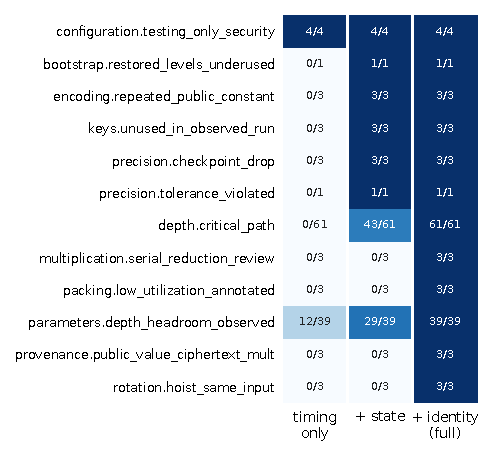
\includegraphics[width=\linewidth]{figures/ablation.pdf}
  \caption{Which part of the trace each rule needs. The same seeded runs are
  re-analyzed under three progressively richer views; cells show positives
  recovered out of positives available. One rule survives on timings alone;
  six require ciphertext version identity. This is an ablation of
  CipherScope's own trace, not a run of an external profiler.}
  \label{fig:ablation}
\end{figure}

\subsection{RQ3: Precision on real findings}
\label{sec:rq3b}

Twelve findings came out of the CKKS corpus. Four are depth-critical-path
reports, which are informational---the rule fires whenever lineage
exists---so they carry no precision denominator; the remaining eight split
six actionable true positives to two false positives.

The two false positives are worth more than the six hits, and they fail
differently. One is a limitation we cannot fix at this observation
boundary: the rule reported headroom, but both reduced depths abort inside a
two-iteration \texttt{EvalBootstrap} whose internal level consumption no
ciphertext state exposes. The other was a defect we could fix: the reported
headroom did not exist because the final ciphertext carried a deferred
rescale, committing one more level than the level field showed. That
diagnosis became a rule change---the depth rule now reserves a
pending-rescale level---and the rule reports that run clean today. We keep
the adjudicated verdict rather than retroactively crediting the fix, so the
reported precision understates the current rule by one finding. Quoting the
improved number would make the table unreproducible from the archived
verdicts.


\begin{figure}
  \centering
  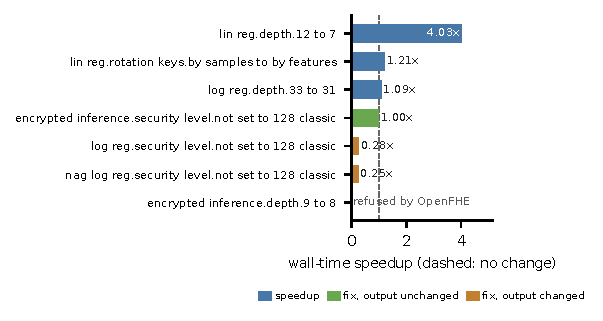
\includegraphics[width=\linewidth]{figures/impact.pdf}
  \caption{Measured outcome of every attempted transformation on the
  external corpus. Enabling standard security enforcement was free on the
  inference workload but cost 3.5--4$\times$ on the two training workloads
  \emph{and changed their numerical results}, because enforcement enlarges
  the ring: the finding is actionable either way, and the trade is the
  developer's. The patch for the adjudicated false positive was refused by
  OpenFHE and is retained as evidence.}
  \label{fig:impact}
\end{figure}

\subsection{RQ4: Impact of acting on findings}
\label{sec:rq4}

A finding that nobody can act on is not a result, so every actionable
finding was patched and measured, with the workload's own correctness check
as the acceptance criterion (Figure~\ref{fig:impact}).

The three performance findings behaved as the rules suggested, the largest
coming from reducing a configured depth of 12 to the 7 actually observed.
The three security findings are more interesting, because enabling standard
128-bit enforcement produced three different outcomes: free on one workload
whose parameters already satisfied the standard ring size, and a
3.5--4$\times$ slowdown on the two training workloads that also
\emph{changed their numerical results}, because enforcement enlarges the
ring. A security fix is not a speedup. What the finding delivers is a
measured trade---security against performance and accuracy---that the
developer is now in a position to make deliberately. The patch attempted for
the adjudicated false positive was refused by OpenFHE at run time, and we
keep it in the figure as evidence of the adjudication rather than deleting
an unflattering row.

A designed suite pairs every prescriptive rule with a minimal program where
the finding fires, a patch following the rule's own suggestion, and a
re-trace that must come back clean or abstaining. All ten pairs behave as
designed. One is a deliberate caution: fixing a testing-only security
configuration makes the toy program roughly four times slower, and the table
says so.


\begin{figure*}
  \centering
  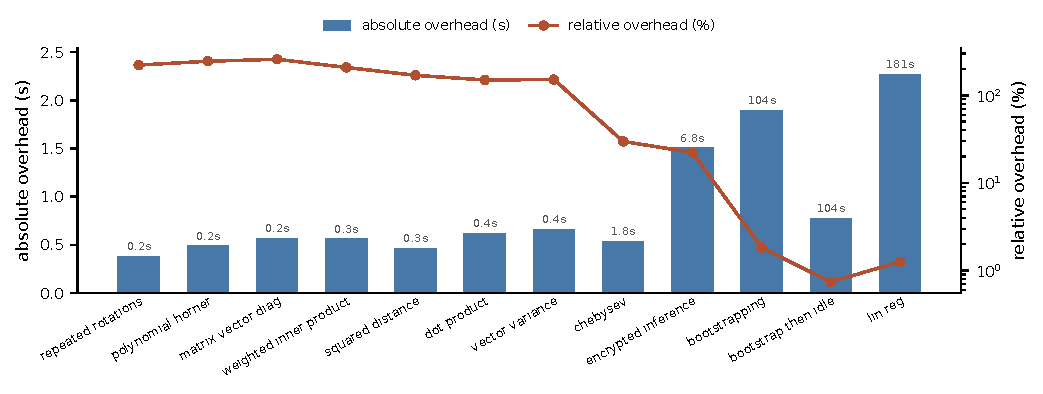
\includegraphics[width=0.92\textwidth]{figures/overhead.pdf}
  \caption{Per-workload tracing cost, sorted by baseline duration. Bars:
  absolute overhead (recording, finalization, and analysis). Line (log
  scale): the same cost relative to the baseline. The absolute cost is
  roughly fixed, so the relative cost falls from a few multiples on
  sub-second examples to under 2\% on workloads of 100\,s or more. Three
  matched repetitions per workload, one machine.}
  \label{fig:overhead}
\end{figure*}

\subsection{RQ5: Cost of tracing}
\label{sec:rq5}

Tracing cost is almost entirely fixed---recording, finalization, and
analysis---so a single pooled ratio would be meaningless. Figure~\ref{fig:overhead}
plots both views: the absolute cost is roughly flat across a twelve-workload
corpus spanning three orders of magnitude in duration, which means the
relative cost falls from a few multiples on sub-second examples to under 2\%
on the workloads anyone would actually profile. CPU overhead on the long
workloads is within noise of zero.

An event-count sweep from $10^2$ to $10^5$ events confirms the shape:
run-phase overhead stays bounded and trace size stays linear at about
2.2\,KB per event. The ceiling is finalization, which is not streamed---at
$10^5$ events, materializing and analyzing the trace peaked at 3.2\,GB
resident. A second limit surfaced while validating on a memory-capped
machine: the deep-bootstrap seeded case peaks near 7\,GB on its own and is
killed below roughly 8\,GB, presenting as a missing bundle rather than an
error message. The artifact documentation names that symptom. Scaling points
are single runs on shared machines, so we treat them as observations rather
than stable estimates.

\subsection{RQ6: Misconfiguration in real programs}
\label{sec:rq6}

Across ten real programs the configuration rule found five declared
testing-only security settings: three in the external suite, all actionable
and all fixed and measured under RQ4, and two in upstream OpenFHE examples
where the setting is deliberate for tractability and was adjudicated
non-actionable. Five programs were clean and none produced a false positive.

The precision rules abstained on all ten, which is the correct answer rather
than an absence of result: unmodified programs declare no checkpoints, so
there is nothing to measure. That abstention is also the honest cost of the
annotation requirement, and we count it here rather than reporting those
rules as silent.

\section{Limitations}
\label{sec:limits}

\paragraph{The observation boundary.} CipherScope sees calls that cross the
application boundary and nothing else: raw-context calls, module-level free
functions, \texttt{GetCryptoContext()} escapes, and native-internal work
are invisible. Coverage classes measure this operationally; they do not
prove completeness. Threshold FHE and proxy re-encryption are outside the
operation manifest today and are rejected by name in strict mode.

\paragraph{Scheme asymmetries.} BFV depth findings are inferences from
recorded operations against a value-dependent noise budget, stated as such
and carrying inferred confidence. Bootstrap analysis requires inputs deeper
than OpenFHE's fixed return level, and is unavailable on the integer
schemes on this build. Precision rules are CKKS-only by construction and
require shadow mode, a secret key, and developer checkpoints.

\paragraph{Evidence limits.} Depth headroom is an upper bound in the
presence of opaque calls, and one of the two real false positives is
exactly that case. Seeded recall is not real-workload recall. Precision
rests on eight adjudicated findings judged by AI reviewers under a fixed
rubric (\S\ref{sec:setup}). The ablation is a projection of CipherScope's
own trace, not a benchmark of an external profiler. The two cluster gate
archives predate the two newest checks. Scaling points are single runs.

\paragraph{Trace sensitivity and security scope.} As stated in
\S\ref{sec:threat}: traces are confidential development artifacts, and
CipherScope makes no cryptographic security claims.

\section{Related Work}
\label{sec:related}

Each neighboring system answers a different question with different
information, and the comparisons below are scoped to that.

\paragraph{Library profilers and benchmark harnesses.}
HEProfiler~\cite{takeshita2025heprofiler} compares the CKKS implementations
of PALISADE, SEAL, HElib, and HEAAN by benchmarking their core operations
across parameter settings, with each library's own maintainers tuning its
parameter selection. The developer writes benchmarks against its C++
framework; it reports no per-call source attribution, no ciphertext lineage,
and no rotation-key accounting, because those are properties of an
application rather than of a library.
CryptOracle~\cite{cryptoracle2025} packages an
OpenFHE benchmark suite with a hardware profiler and a predictive
performance and energy model. Cross-platform and cross-library benchmarks compare schemes and libraries
under fixed workloads~\cite{crossplatform2025,safetycentric2025}, and
architecture-centric studies characterize the kernels below the application
boundary. None of these traces a developer's own program at that boundary,
which is the question CipherScope answers; conversely, CipherScope measures
nothing about library internals or energy.

\paragraph{Language-level profilers.} Scalene~\cite{berger2023scalene}
attributes Python versus native cost, memory, and copying at the language
boundary; Coz~\cite{curtsinger2015coz} estimates the causal effect of
speeding up a line via virtual-speedup experiments. Both answer ``where
does time go, and what would speed things up'' without FHE semantics:
neither can state that two rotations consumed one ciphertext version or
that a rotation key went unused. CipherScope does not attempt their
measurements---it records whole-call times only as context for its semantic
findings, and suggests experiments rather than estimating causal speedups.

\paragraph{FHE compilers and configuration tools.}
EVA~\cite{dathathri2020eva} and HEIR~\cite{heir2025} construct or optimize
FHE programs through compiler representations; HECATE~\cite{hecate2022}
optimizes CKKS scale management with a latency-aware planner;
Rotom~\cite{rotom2026} derives packing layouts; their analyses are static
over an intermediate representation. FHE-Agent~\cite{fheagent2025} searches
the CKKS configuration space with an LLM controller over deterministic
profiling tools; it selects parameters for a model it is given, whereas
CipherScope diagnoses a program as written and configured. CipherScope's
graph is the \emph{executed} run of an already-written program---it
observes taken branches, runtime-chosen parameters, and library behavior as
shipped, and it rewrites nothing. The approaches are complementary: a
compiler could consume facts CipherScope observes, and several of its
diagnoses (hoisting, layout) correspond to transformations compilers
perform when the program is written in their input language.

\paragraph{FHE testing and implementation security.}
HERTA~\cite{herta2026} metamorphically tests FHE frameworks using generated
programs; it targets library correctness, not application diagnosis.
Implementation-security analyses of FHE libraries (memory safety, side
channels) operate below the application boundary and are complementary to
the configuration-level observations CipherScope makes
(\S\ref{sec:threat}).

\section{Conclusion and Future Work}
\label{sec:conclusion}

CipherScope demonstrates that application-level FHE execution can be
observed precisely enough to support conservative, evidence-carrying
diagnoses---across three schemes, two languages, and four evidence
lanes---and that the observations are worth having: on an independently
authored corpus, six of eight adjudicated findings were actionable, and
acting on them produced measured improvements up to 4.03$\times$ alongside
measured security--performance trades. The methodology may travel further
than the tool: measured observation boundaries, known-answer benchmarks
with hard negatives and abstention assertions, adjudication with preserved
false positives, and byte-reproducible tables are applicable to any FHE
tooling claim.

Future work follows the measured gaps. The threshold-FHE and
proxy-re-encryption families that rejected three of five integer-scheme
workloads are the next coverage frontier; streaming finalization would
remove the known memory ceiling; human re-adjudication would strengthen the
precision evidence; and the two cluster lanes await a rerun at the full
check count. The artifact contains every raw record, checksum, patch, and
regeneration command behind every number in this paper.

\bibliographystyle{ACM-Reference-Format}
\bibliography{references}

\end{document}
